\documentclass[11pt,twoside,a4paper]{article}
\usepackage{cite}
\usepackage[cm]{fullpage}
\usepackage{graphicx}
\usepackage{feynmp}
\usepackage{amsmath}
\usepackage{amssymb}
\DeclareGraphicsRule{*}{mps}{*}{}
\usepackage{caption}
\usepackage{subcaption}
\usepackage{slashed}
\usepackage[utf8]{inputenc}


\begin{document}
\begin{fmffile}{feynmandiags}

\title{Higgs boson searches and Higgs decays to invisible final states at the Compact Muon Solenoid}
\author{Patrick Dunne \\ Supervisors: David Colling, Gavin Davies}
\maketitle


\renewcommand{\abstractname}{\vspace{-\baselineskip}}
\begin{abstract}
  An overview of searches for the Higgs boson at the Compact Muon Solenoid (CMS) at the Large Hadron Collider (LHC) is presented. A particular emphasis is placed on the methods of combining the various decay channels that are used and the search for invisible Higgs boson final states in the vector boson fusion (VBF) production channel.
\end{abstract}


\section{The Standard Model and the Higgs boson}
\label{theory}

The Standard Model (SM) of particle physics is one of the most successful physical theories devised, and one of its cornerstones is electroweak unification \cite{glashow,weinberg,salam}. Electroweak unification proposes that the Lagrangian has an SU(2)xU(1) symmetry and local gauge invariance with four gauge bosons, the photon ($\gamma$) and the $W$ and $Z$ bosons. The particles predicted by the theory, the $W$ and $Z$ bosons, were observed at the UA1 and UA2 experiments in 1983 \cite{wdiscovery,zdiscovery}, with masses of 80.4 GeV and 91.2 GeV, respectively. It was already known that massive exchange particles would be required to explain the short range of the weak force. Unfortunately the symmetry of the Lagrangian is ruined by vector boson mass terms, so a different mechanism is required to give mass to the particles we observe.

The Higgs mechanism provides a solution to this problem by adding a complex scalar field with a non-zero vacuum expectation value, the Higgs field, to the Lagrangian that couples to the gauge bosons \cite{englertbrout,higgs1,higgs2,guralniketc,higgs3,kibble}. While the Lagrangian term itself respects the symmetry described above, the ground state does not; this is called spontaneous symmetry breaking. The gauge bosons coupling to a field with a vacuum expectation accounts for their mass, and we are left with the prediction of a new massive scalar boson, the Higgs boson. A candidate Higgs-like boson has recently been discovered by the ATLAS and CMS \cite{cmsdiscovery,atlasdiscovery} experiments at CERN.

The Higgs mechanism can also explain the fermion masses by introducing a Yukawa coupling between the Higgs field and the fermions, the mass would be expected to be proportional to the strength of the coupling. Measuring the strength of the coupling between the Higgs-like boson that has been discovered at the LHC \cite{lhc} and the fermions will therefore be important in confirming whether it is a SM Higgs boson. It is important to note that the theory does not predict the particles' masses.

\begin{figure}
  \centering
  \raisebox{-0.5\height}{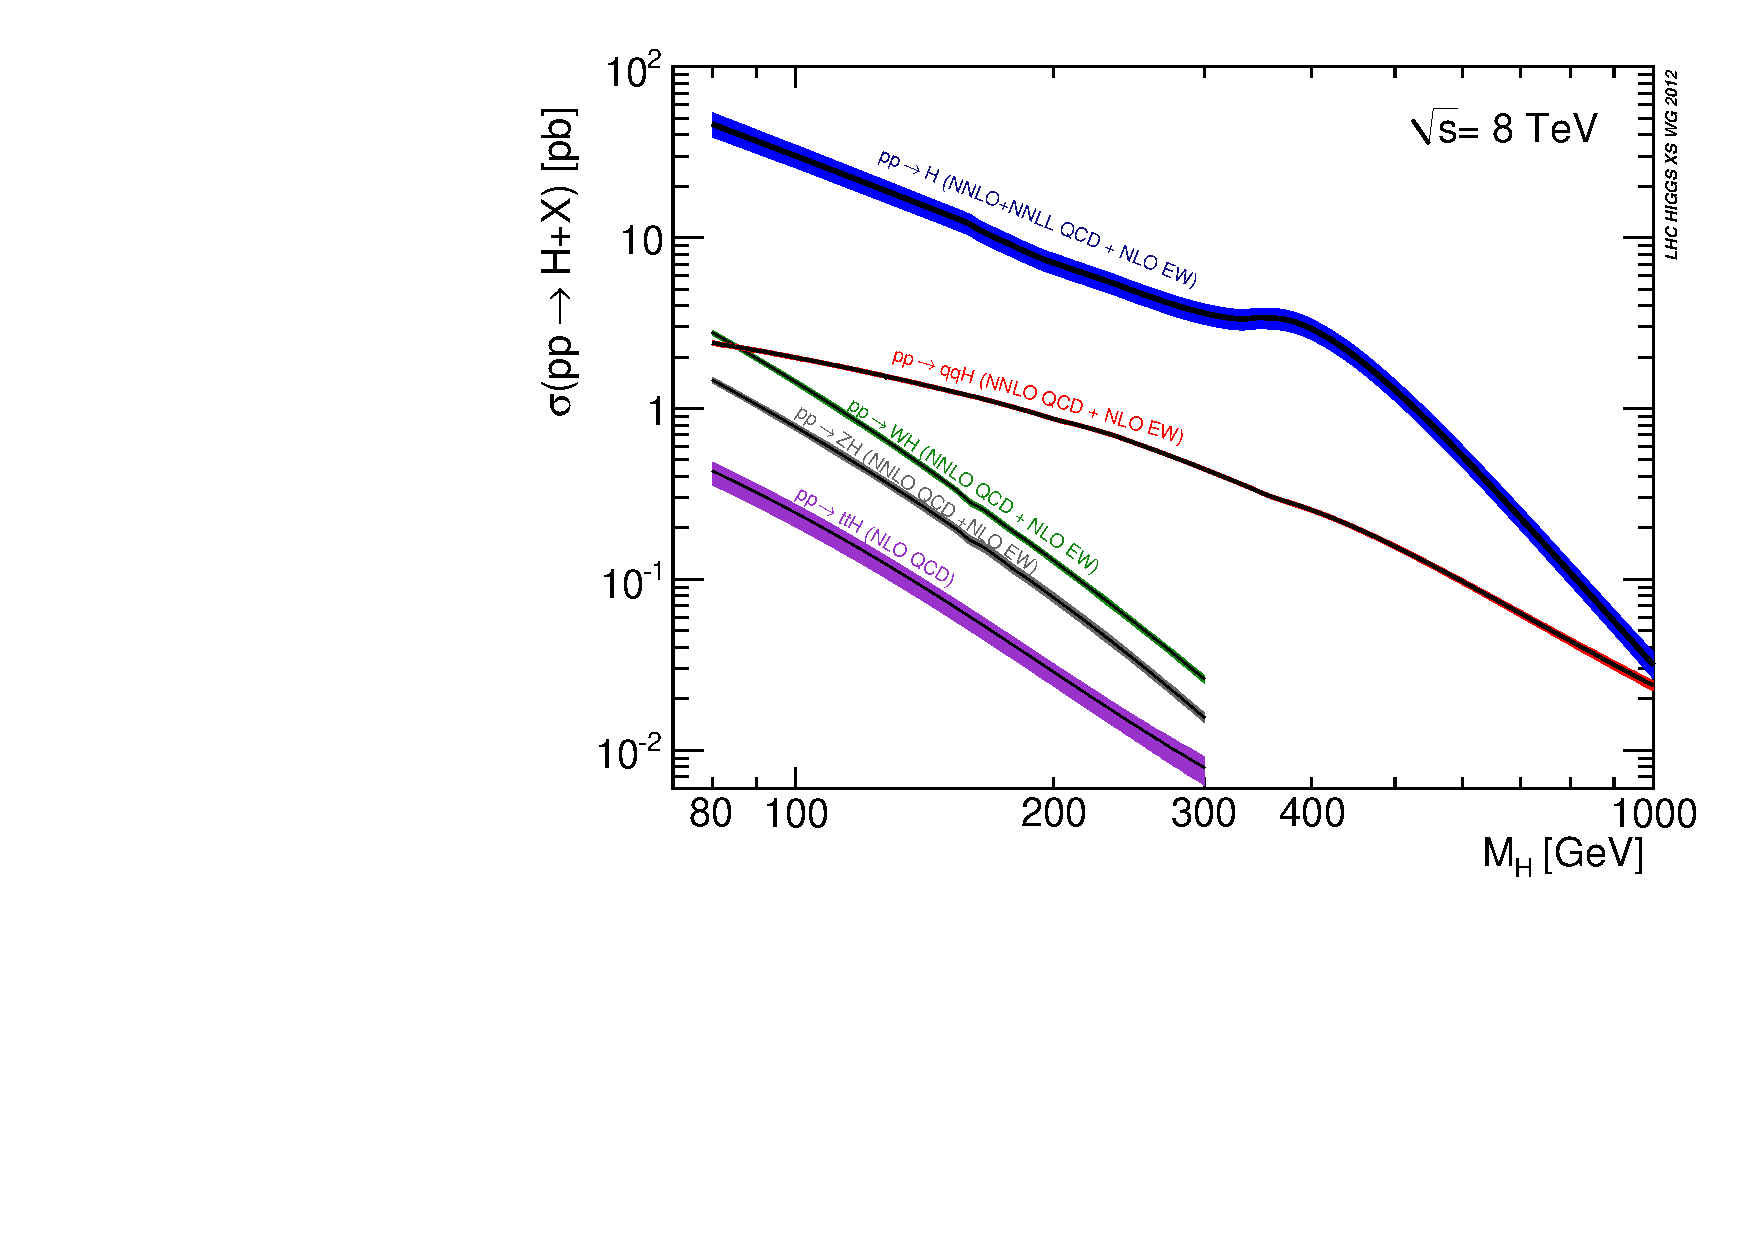
\includegraphics[width=0.49\textwidth]{Higgs_XS_8TeV_lx.pdf}}
  \raisebox{-0.5\height}{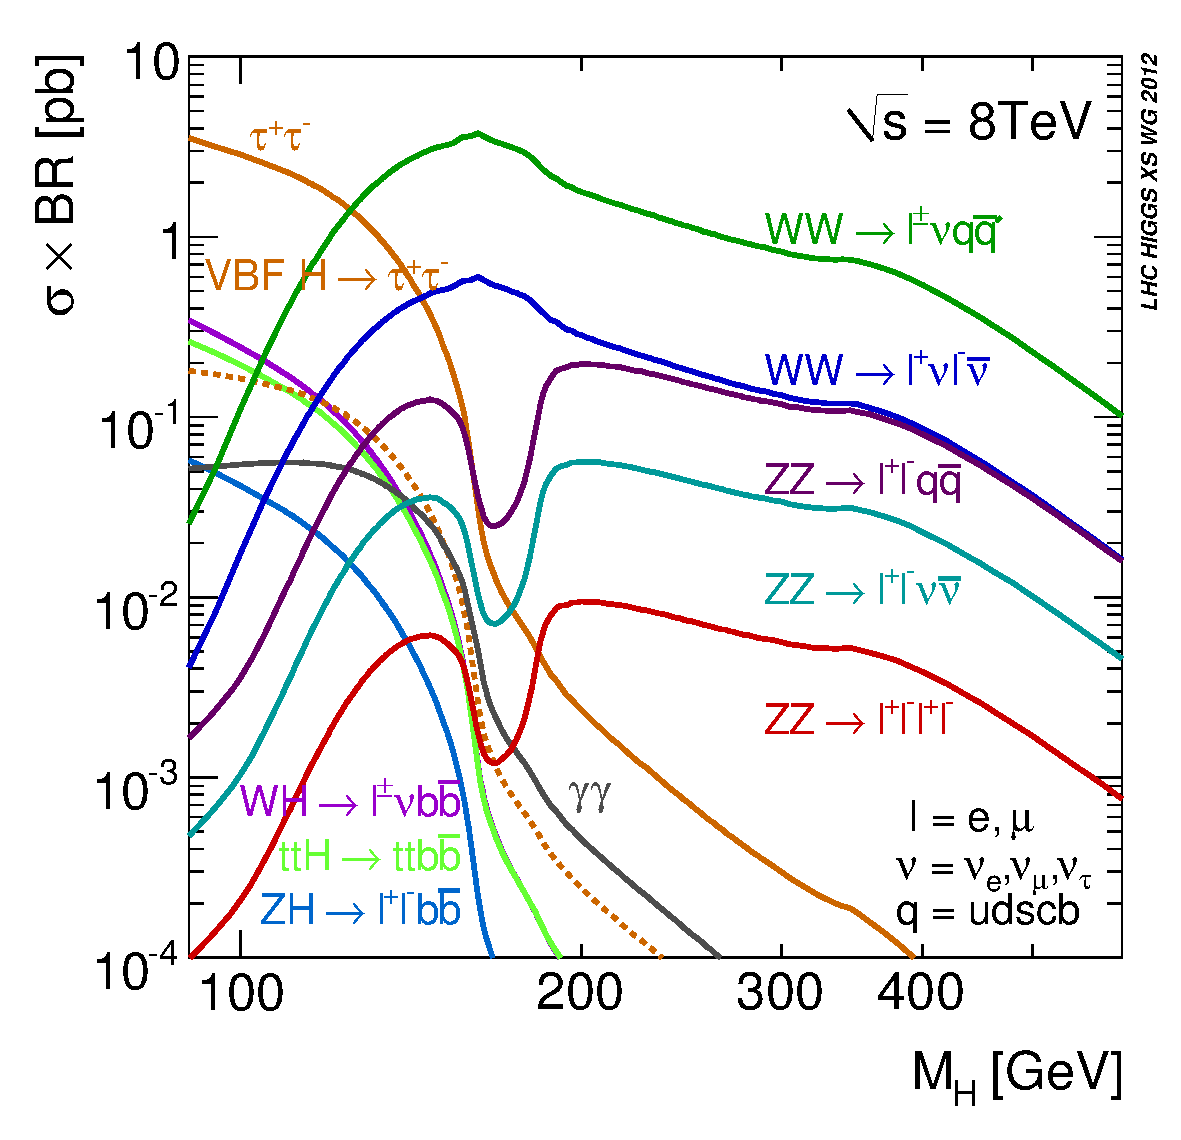
\includegraphics[width=0.49\textwidth]{XSBR_8TeV_SM.pdf}}
  \caption{Cross-section for SM Higgs boson production mechanisms is shown (left), $pp \rightarrow H$ is gluon fusion, $pp \rightarrow qqH$ is VBF and the remaining three are associated production with $W$, $Z$ and $t\bar{t}$. Also shown (right) are the branching fractions multiplied by the production cross-section for the decay modes of the SM Higgs boson. From \cite{lhchxswg}}.
  \label{higgbrfig}
\end{figure}


\begin{figure}
  \centering
  \begin{subfigure}{0.24\textwidth}
    \centering
    %ggf 
    \begin{fmfgraph*}(75,100)
      \fmfleft{i0,i1,i2,i3,i4,i5}
      \fmfright{o1}
      \fmf{gluon}{i1,v1}
      \fmf{gluon}{i4,v2}
      \fmf{fermion,tension=0}{v1,v2}
      \fmf{fermion,tension=2/3}{v2,v3,v1}
      \fmf{dashes}{v3,o1}
      \fmflabel{$g$}{i1}
      \fmflabel{$g$}{i4}
      \fmflabel{$H$}{o1}
    \end{fmfgraph*}
    \caption{}
  \end{subfigure}
  \begin{subfigure}{0.24\textwidth}
    \centering
    %vbf                                                                                                   
    \begin{fmfgraph*}(75,100)
      \fmfleft{i1,i2}
      \fmfright{o1,o2,o3}
      \fmf{fermion}{i1,v1,o1}
      \fmf{fermion}{i2,v2,o3}
      \fmf{photon,label=$W,,Z$}{v1,v3}
      \fmf{photon,label=$W,,Z$}{v2,v3}
      \fmf{dashes}{v3,o2}
      \fmflabel{$q$}{i1}
      \fmflabel{$q$}{i2}
      \fmflabel{$q$}{o1}
      \fmflabel{$q$}{o3}
      \fmflabel{$H$}{o2}
    \end{fmfgraph*}
    \caption{}
  \end{subfigure}
  \begin{subfigure}{0.24\textwidth}
    \centering
    %Higgstrahlung
    \begin{fmfgraph*}(75,100)
      \fmfleft{i1,i2}
      \fmfright{o1,o2}
      \fmf{fermion}{i1,v1}
      \fmf{fermion}{v1,i2}
      \fmf{photon,label=$W,,Z$}{v1,v2}
      \fmf{photon}{v2,o1}
      \fmf{dashes}{v2,o2}
      \fmflabel{$q$}{i1}
      \fmflabel{$\bar{q}$}{i2}
      \fmflabel{$W,Z$}{o1}
      \fmflabel{$H$}{o2}
    \end{fmfgraph*}
    \caption{}
  \end{subfigure}
  \begin{subfigure}{0.24\textwidth}
    \centering
    %ttH                                                                                                    
    \begin{fmfgraph*}(75,100)
      \fmfleft{i0,i1,i4,i5,i6,i2,i3}
      \fmfright{o0,o1,o2,o3,o4}
      \fmf{gluon,tension=3/2}{i1,v1}
      \fmf{gluon,tension=3/2}{i2,v2}
      \fmf{fermion}{o1,v1,v3,v2,o3}
      \fmf{dashes,tension=3/2}{v3,o2}
      \fmflabel{$g$}{i1}
      \fmflabel{$g$}{i2}
      \fmflabel{$\bar{t}$}{o1}
      \fmflabel{$t$}{o3}
      \fmflabel{$H$}{o2}
    \end{fmfgraph*}
    \caption{}
  \end{subfigure}
  \caption{The Feynman diagrams for the Higgs production mechanisms at CMS are shown: a) gluon gluon fusion, b) vector boson fusion, c) $W$/$Z$ associated production and d) $t\bar{t}$ associated production.}
  \label{higgprodfig}
\end{figure}

\section{Higgs production and decay mechanisms}
\label{proddec}

As can be seen in Fig.~\ref{higgbrfig} the SM Higgs boson production mechanism with the highest cross-section at the LHC is gluon gluon fusion which proceeds through a quark loop as shown in Fig.~\ref{higgprodfig}a. Because the Higgs couples to mass this loop is dominated by the top quark contribution, although all strongly interacting massive particles are expected to contribute.

After gluon gluon fusion the next highest production cross-section is for vector boson fusion (VBF), which occurs through the Feynman diagram shown in Fig.~\ref{higgprodfig}b. VBF has the advantage that the two quarks in the final state are produced with a large pseudorapidity (defined in Sec. \ref{cmslhc}) gap between them, which can be used as a signature to trigger on \cite{zeppenfeld}.

Finally there is associated production, where the Higgs is produced along with other particles, predominantly $W$ or $Z$ bosons and $t\bar{t}$ pairs through the diagrams in figs. \ref{higgprodfig}c and \ref{higgprodfig}d. These channels are useful because the particles produced with the Higgs can be used for triggering, thus reducing backgrounds.

As described above the Higgs boson couples proportionally to mass, so it would be expected that the dominant decays would be to heavy particles. At a mass around 125 GeV the heaviest particle that can be pair produced on-shell is the b quark. However, large QCD backgrounds make it impossible to perform a Higgs search in the $b\bar{b}$ channel unless the Higgs was created in associated production, when the associated particle can be used as a trigger, and the background is significantly reduced.

As the mass increases decays to two $W$ or $Z$ bosons become increasingly important. It can be seen from Fig.~\ref{higgbrfig} that both the $WW$ and $ZZ$ channels have high branching ratios even at 125 GeV, because, even though two real bosons cannot be created, it is possible to produce one real and one virtual boson. When at least one of the bosons decays leptonically the lepton can be used to trigger allowing this search to be carried out for all of the production channels. The $ZZ$ channel is also particularly important because several of its final states allow full kinematic reconstruction giving it a very good mass resolution.

The other channel with very good mass resolution is the decay to two photons ($\gamma\gamma$), which also has a final state that can be fully reconstructed and is easy to trigger on. The $\gamma\gamma$ decay proceeds through a similar loop diagram to gluon gluon fusion, but with the gluons replaced with photons and any massive charged particle in the loop. The $\gamma\gamma$ decay also has most sensitivity at low mass because at higher masses decays to $WW$, $ZZ$ and, at very high Higgs mass, $t\bar{t}$ are dominant. 

The final channel that is being examined for the main Higgs search at CMS is the decay to two $\tau$ leptons. Fig.~\ref{higgbrfig} shows that this has a high branching ratio, however the fact that when the $\tau$ leptons decay neutrinos are produced with variable energies means that this channel does not have a good mass resolution. The signal of a decay to two $\tau$ leptons therefore manifests itself as a broad excess which is difficult to search for. Like the $\gamma\gamma$ channel the decay to $\tau$ leptons is also a channel with most sensitivity in the low mass region.

Whilst the SM branching fraction is vanishingly small, there are also searches for Higgs decays to invisible final states because several beyond the SM models predict Higgs decays to long-lived neutral particles. Decays to invisible final states (``Higgs to invisible'') are studied in more detail in Sec. \ref{htoinv}

\section{CMS and the LHC}
\label{cmslhc}
The LHC is a proton proton collider situated at CERN near Geneva with nominal centre of mass energy ($\sqrt{s}$) of 14 TeV. It ran in 2010 and 2011 at $\sqrt{s}$ = 7 TeV, and again in 2012 at $\sqrt{s}$ = 8 TeV. The CMS detector is one of the two general purpose detectors at the LHC, the other being ATLAS. From the inside out it comprises: a central silicon detector for vertex location and tracking, an electromagnetic calorimeter (ECAL), a hadronic calorimeter (HCAL), a superconducting magnet to bend particle tracks for momentum measurement and a muon system situated in the magnet return yoke\cite{cmstdr}.

The co-ordinate system used by CMS is right-handed with the x-axis pointing to the centre of the LHC ring, the y-axis pointing vertically upwards and the z axis along the beam-line. The spherical polar co-ordinates $\theta$ and $\phi$ take their normal definitions. CMS also uses the pseudorapidity variable, $\eta$, which is defined as
\begin{equation}\label{pseudorap}
  \eta = -\ln\tan(\frac{\theta}{2}).
\end{equation}

All the subdetectors cover the full $2\pi$ range in $\phi$, except for small regions blocked by services such as power cabling and cooling. The pseudorapidity ranges of the subdetectors vary and will be described below.

The tracker consists of an inner pixel detector and an outer silicon strip detector. Both the pixel and strip detectors are split into a barrel section and endcaps and cover the pseudorapidity range $|\eta| < 2.5$. The pixel detector has a resolution  of ~15 $\mu$m in r-$\phi$ and z giving vertex resolutions of 30-40 $\mu$m in the longitudinal direction, while the strip detector has a resolution in the range 23-52 $\mu$m in r-$\phi$ and 230-530 $\mu$m in z \cite{detthesis}. This high accuracy is necessary to discriminate between tracks from pileup (particles from interactions other than the interaction of interest) and the collision of interest; it also improves the energy resolution of objects reconstructed by matching calorimeter deposits to tracks. The tracker determines particle momentum from the curvature of tracks, achieving a resolution of 1-2\% for 100 GeV particles with $\eta<1.6$ \cite{cmstdr}.

The ECAL is a homogeneous PbWO$_{4}$ scintillating calorimeter which is split into a barrel section and an endcap section and covers the pseudorapidity range $|\eta|<3.0$. Its energy resolution is energy dependent and is well described by:
\begin{equation}\label{sigmaE}
  \frac{\sigma}{E} = \frac{\alpha}{\sqrt{E}}\sqrt{\rm{GeV}} \oplus \frac{\beta}{E}\rm{GeV} \oplus \delta\,.
\end{equation}
with $\alpha$ = 2.8\%, $\beta$ = 0.12 and $\delta$ = 0.3\% \cite{detthesis}. The ECAL energy resolution is important in determining the accuracy of any missing energy calculation, making it key to Higgs to invisible searches. The sensitivity of the Higgs to $\gamma\gamma$ channel is also very dependent on good ECAL energy resolution.

The HCAL is made up of a barrel region and endcaps, covering $|\eta| < 3.0$, and a forward region, covering $3.0<|\eta|<5.0$. The barrel and endcaps are sampling calorimeters composed of interleaved brass and plastic scintillator. The forward HCAL is a steel and Cherenkov emitting quartz fibre sampling calorimeter. The energy resolution of the HCAL and ECAL combined, which is the figure most important for missing energy determination, is well described by Eq. \ref{sigmaE} with $\alpha$=1.21 GeV$^{1/2}$, $\beta$=0.095 and $\delta$=0 \cite{detthesis}. The forward HCAL is particularly important for the Higgs to invisible search, and any other VBF processes, because the large pseudorapidity gap expected means that 80\% of VBF events with a pseudorapidity gap of at least 4.4 will have at least one jet in the forward HCAL \cite{higgworkgroup2001}.

The muon system is situated in the return yoke of the superconducting magnet and consists of a drift tube system in the barrel section of the detector, a cathode strip chamber system in the endcap and a resitive plate chamber system both in the endcaps and the barrel. Together these systems cover the pseudorapidity range $|\eta|<2.4$. Combined with inner tracker information the muon system gives a momentum resolution of $\delta p_{T}$/$p_{T}$ between 0.01 and 0.1 for muons with $p_{T}$ between 10 and 1000 GeV.

To date an integrated luminosity of 5.6 fb$^{-1}$ has been recorded by CMS at $\sqrt{s}$ = 7 TeV, and 21.8 fb$^{-1}$ have been collected at $\sqrt{s}$ = 8 TeV. However, the rate of collisions at the LHC is too great for CMS to record every detected event; a triggering process is therefore necessary to select the most interesting events for recording. At CMS the trigger consists of the level one trigger which is hardware based, and the higher level trigger (``HLT'') which is software based \cite{detthesis}.

For the 2012 run it was realised that whilst it is only possible to process events at a rate of 700 Hz an extra 1000 Hz could be stored to tape for later processing \cite{parkeddata}. This extra data is referred to as ``parked data'' and is of particular relevance to the Higgs to Invisible search discussed in Sec. \ref{htoinv}.


\section{Higgs to invisible}
\label{htoinv}
In several beyond the SM theories the Higgs boson is expected to have a significant branching ratio for decays to particles that would be invisible to the CMS detector \cite{higgworkgroup2001}. The basic idea is to observe these Higgs to invisible events by using the distinctive VBF Higgs production process topology to tag Higgs events and then searching for missing energy \cite{zeppenfeld}. The VBF channel has been shown to be the most sensitive production channel to decays to invisible final states; this is because of its high cross-section compared to the associated production channels and its more distinctive topology compared to gluon fusion \cite{bds}.

In addition to the gap in pseudorapidity, jets produced in VBF processes are expected to be in opposite halves of the detector. Furthermore, QCD backgrounds can be significantly suppressed whilst retaining high signal efficiency by requiring a high dijet invariant mass \cite{zeppenfeld}. CMS has a dedicated trigger for this analysis which requires two jets and the following other conditions:
\begin{equation}E_{T_{j_{1,2}}} >40\,\rm{GeV}, \eta_{j_{1}} \cdot \eta_{j_{2}} < 0, \Delta\eta_{jj} > 3.5, M_{jj} > 800\,\rm{GeV}, \slashed{E}_{T} > 65\,\rm{GeV},
\end {equation}
 where $\slashed{E}_{T}$ is the missing transverse energy. Other than the missing $E_{T}$ trigger, which is specific to invisible decays, these are generic cuts for VBF analyses \cite{jimtalk}.

Even after selecting for the VBF topology and missing energy, there are still significant backgrounds to a Higgs to invisible search. Both $Z$ + jets and $W$ + jets where the leptons are missed have missing energy and can occur via VBF and thus also have the same pseudorapidity gap. Further backgrounds are expected from mismeasured QCD events which give fake missing energy. $W$ + jets and $Z$ + jets also occur via QCD and produce further backgrounds \cite{bds}. Further offline cuts are made and take the form of:
\begin{equation}E_{T_{j_{1,2}}} > 50 \,\rm{GeV}, \eta_{j_{1}} \cdot \eta_{j_{2}} < 0, |\eta_{j_{1,2}}| < 4.7, \Delta\eta_{jj} > 4.2, M_{jj} > 1200 \,\rm{GeV}, \slashed{E}_{T} > 130 \,\rm{GeV}.
\end{equation}
These cuts significantly reduce the QCD backgrounds \cite{zeppenfeld}, however the $W$ + jets and $Z$ + jets backgrounds remain; while these two backgrounds are mostly indistinguishable from the signal they do have a significant difference in the distribution of azimuthal angle between the VBF jets. For Higgs events the jets are expected to be very close to each other in azimuthal angle, whereas for $W$ and $Z$ events the jets are expected to be opposite to each other. A cut of $\Delta\phi_{jj}<1$ is therefore made.

Remaining backgrounds are estimated from control regions which are $Z \to \mu\mu$ decays for the $Z$ + jets background, $W$ + jets + identified leptons for the case of the $W$ + jets with missed leptons background and the high $\Delta\phi_{jj}$ region for QCD background \cite{jimtalk}.

At present, analysis of the data from the 2012 LHC run is taking place, and it is envisaged that in the near future the analysis will be performed using the parked data discussed in Sec. \ref{cmslhc}. The triggers present in the parked data are less stringent, the $\slashed{E}_{T}$ threshold is lowered to 35 GeV, the $E_{T}$ threshold is lowered to 35 GeV and the $M_{jj}$ threshold is lowered to 700 GeV, which should result in fewer signal events being lost \cite{jimtalk}. More work is also required to investigate the possibility of vetoing events with jet activity in the central region, which would further reduce backgrounds.


\section{Combination of Higgs boson decay channels}
\label{combs}
In order to establish whether what has been found at CMS is an SM Higgs boson it is important to combine the results of the different searches and compare them with the SM predictions. In order to do this the errors, both statistical and systematic, on the various analyses and their correlations must be taken into account as well as each channel's results.

The CMS combinations group compares the data to standard model predictions in three main ways: limits are placed on regions where we can exclude a standard model Higgs boson, excesses over background are characterised and signal model parameters are extracted and compared to their standard model values \cite{hcpcomb2012}. A general methodology for doing this has been developed by ATLAS and CMS which is described in refs. \cite{lhccomb1,comb2011} and described below are the methods used for performing the above three data to signal comparisons as they appear in ref. \cite{hcpcomb2012}.


\subsection{Exclusion limits}
For setting exclusion limits the CL$_{s}$ statistic is used, which is a function of the profile likelihood ratio, q$_{\mu}$, defined as:
\begin{equation}
  q_{\mu} = -2 \ln\frac{\mathcal{L}(obs|\mu \cdot s + b,\hat{\theta}_{\mu})}{\mathcal{L}(obs|\hat{\mu} \cdot s + b,\hat{\theta})}\,,
\end{equation}
where s is the SM expected Higgs signal and b is the background. $\mu$ is a signal strength modifier which is 1 for a SM Higgs boson and 0 for the background only case. $\theta$ are nuisance parameters, such as systematic errors, which include the errors and any correlations between them. $\hat{\mu}$ and $\hat{\theta}$ are the values of $\theta$ and $\mu$ where the likelihood, $\mathcal{L}$, is maximised, and $\hat{\theta}_{\mu}$ is the $\theta$ that maximises the likelihood for a given $\mu$. The profile likelihood ratio therefore describes how likely a given signal strength is compared to the most likely signal strength.

The definition of CL$_{s}$ is
\begin{equation}
  CL_{s} = \frac{P(q_{\mu}\geqslant q_{\mu}^{obs} | \mu \cdot s + b)}{P(q_{\mu}\geqslant q_{\mu}^{obs}|b)}\,,
\end{equation}
Where the method of the determining probability, $P$ ,varies. The region in which a signal strength $\mu \cdot s$ is excluded with $1 - \alpha$ confidence is then the region for which CL$_{s}$ is less than or equal to $\alpha$ i.e. when the background hypothesis is $1/\alpha$ times more likely than the signal hypothesis we exclude the signal hypothesis with $1 - \alpha$ confidence.

\subsection{Characterising excesses}
When the signal model cannot be excluded, the observed excess of events over that expected from background is characterised by calculating q$_{0}$ by setting $\mu$ to zero in q$_{\mu}$. Next, p$_0$, which is defined as
\begin{equation}
p_{0} = P(q_{0} \leqslant q_{0}^{obs}|b)\,,
\end{equation}
is calculated and then the statistical significance of the excess, Z in units of standard deviations, is defined as the value of Z for which:
\begin{equation}
  p_{0}=\int_{Z}^{+\infty}\frac{1}{\sqrt{2\pi}}\exp(-x^{2}/2)dx\,.
\end{equation}

\subsection{Signal parameter determination}
In order to extract confidence limits on signal model parameters the profile likelihood ratio is used again, in this case it is defined as:
\begin{equation}
  q(a) = -2\ln\frac{\mathcal{L}(obs|s(a)+b,\hat{\theta}_{a})}{\mathcal{L}(obs|s(\hat{a})+b,\hat{\theta})}\,,
\end{equation}
where a is the parameter of interest, s, b and $\theta$ are defined as above, $\hat{a}$ and $\hat{\theta}$ are the values of $\theta$ and a at the global maximum of $\mathcal{L}$ and $\hat{\theta}_{a}$ is the $\theta$ that maximises $\mathcal{L}$ for the given a.

The one sigma and two sigma confidence limits on the parameter are then the values of a for which q(a) is equal to 1.00 or 3.84 respectively treating all other unconstrained parameters as nuisance parameters. It is also possible to produce confidence limit contours for two parameters by taking q($a_{i}$,$a_{j}$), however the values of q corresponding to one sigma and two sigma contours are now 2.30 and 6.00 respectively.

\subsection{Results of previous searches}
The first CMS Higgs combination paper \cite{comb2011} was published on the 2011 data which were taken at $\sqrt{s}$=7 TeV and corresponded to an integrated luminosity of 4.6-4.8 fb$^{-1}$. At 95\% confidence level Higgs boson masses from 127-600 GeV were ruled out, combined with the 114 GeV lower limit set by LEP this was a very strong restriction of parameter space. Furthermore a 2.1$\sigma$ excess (after accounting for the look elsewhere effect) over the background hypothesis was observed in the unexcluded region.

Confirmation of the excess was provided in 2012 when the full 5.1 fb$^{-1}$ of 2011 7 TeV data and 5.3 fb$^{-1}$ of 8 TeV 2012 data were analysed. The 95\% confidence limit for Higgs boson mass exclusion was extended to include the region between 110.0 and 121.5 GeV and a 5$\sigma$ excess was seen in the range 121.5-128 GeV. Using the good resolution channels, described in Sec. \ref{proddec}, the mass was determined to be 125.3 $\pm$ 0.4 (stat.) $\pm$ 0.5 (syst.) GeV. At 125 GeV the extracted value of the SM signal strength modifier is 0.87 $\pm$ 0.23, consistent with the standard model \cite{cmsdiscovery}.

An update of the result which also used an additional 6.9 fb$^{-1}$ of 8 TeV data from the 2012 run was presented at the HCP conference \cite{hcpcomb2012} and showed that the significance of the excess had increased to 6.9$\sigma$. Furthermore extraction of signal parameters still showed no significant deviations from the standard model. Tests of the 0$^{-}$ and 0$^{+}$ spin-parity hypotheses were also made using the Higgs to $ZZ$ to 4 leptons channel. The 0$^{+}$ hypothesis (which is that expected in the SM) was found to be consistent with the data, and the 0$^{-}$ hypothesis was found to be disfavoured, giving a CL$_{s}$ value of only 2.4\%.


\section{Future work}
My thesis will focus on searches for Higgs boson decays to invisible final states in the VBF channel, particularly how these results impact the combination of all the decay channels for determination of the overall parameters of the Higgs boson. I will begin by assisting with the combinations for the Moriond 2013 conference and the analysis of the 2012 data for the Higgs to invisible searches. I will then move on to using the parked data from 2012 for the Higgs to invisible search; this is of particular importance as the LHC is shut down as of mid-February 2013 for two years, so the parked data will be the only available unanalysed data.

Depending on the outcome of this work I will also study the impact of the Higgs to invisible searches on the combinations and preparations for analyses after the shutdown.


\begin{thebibliography}{999}

\bibitem{glashow}S. Glashow, ``Partial-symmetries of weak interactions'', Nucl. Phys. 22 (1961) 579.
\bibitem{weinberg}S. Weinberg, ``A Model of Leptons'', Phys. Rev. lett. 19 (1967) 1264.
\bibitem{salam}A. Salam, ``Weak and electromagnetic interactions,'', in: N. Svartholm (Ed.), Elementary Particle Physics: Relativistic Groups and Analyticity, Prodeedings of the Eighth Nobel Symposium, Almquvist and Wiskell, 1968, p. 367.
\bibitem{wdiscovery} UA1 Collaboration, ``Experimental observation of isolated large transverse energy electrons with associated missing energy at $\sqrt{s} = 540\,\rm{GeV}$,'' Phys. Lett. B122 (1983) 103. 
\bibitem{zdiscovery} UA1 Collaboration,  ``Experimental Observation of Lepton Pairs of Invariant Mass Around 95 GeV at the CERN SPS Collider'', Phys. Lett. B126 (1983) 398. 
\bibitem{englertbrout} F. Englert, R. Brout, ``Broken Symmetry and the Mass of Gauge Vector Mesons'', Phys. Rev. Lett. 13 (1964) 321.
\bibitem{higgs1} P.W. Higgs, ``Broken symmetries, massless particles and gauge fields'', Phys. Lett. 12 (1964) 132.
\bibitem{higgs2} P.W. Higgs, ``Broken Symmetries and the Masses of Gauge Bosons'', Phys. Rev. lett. 13 (1964) 508.
\bibitem{guralniketc} G. Guralnik, C. Hagen, T.W.B. Kibble, ``Global Conservation Laws and Massless Particles'', Phys. Rev. Lett. 13 (1964) 585.
\bibitem{higgs3} P.W. Higgs, ``Spontaneous Symmetry Breakdown without Massless Bosons'', Phys. Rev. 145 (1966) 1156.
\bibitem{kibble} T.W.B. Kibble, ``Symmetry breaking in non-Abelian gauge theories'', Phys. Rev. 155 (1967) 1554.
\bibitem{atlasdiscovery} ATLAS Collaboration, ``Observation of a new particle in the search for the Standard Model Higgs boson with the ATLAS detector at the LHC'', Phys. Lett. B716 (2012) 1.
\bibitem{cmsdiscovery} CMS Collaboration, ``Observation of a new boson at a mass of 125 GeV with the CMS experiment at the LHC'', Phys. Lett. B 716 (2012) 30.
\bibitem{lhc} L. Evans, P. Bryant (Eds.), ``LHC Machine'', JInst. 3 (2008) S08001.
\bibitem{cmstdr} CMS Collaboration, ``The CMS experiment at the CERN LHC'', JInst. 3 (2008) S08004.
\bibitem{detthesis} Anastasios Papageorgiou, CERN Thesis-2010-223.
\bibitem{higgworkgroup2001} Girolamo et al, ``The Higgs Working Group: Summary report, C. Experimental Observation of an invisible Higgs Boson at LHC'', arXiv:hep-ph/0203056 (2001).
\bibitem{parkeddata} Z. Demiragli, CMS triggers for some ``Unexpected Higgs Decays'', Higgs-Exo Workshop 04/02/2013.
\bibitem{bds} Y. Bai et al, ``Measuring the Invisible Higgs Width at the 7 and 8 TeV LHC'', arXiv:1112.4496.
\bibitem{zeppenfeld} D. Zeppenfeld, ``Observing an invisible Higgs boson'', Phys. Lett. B 495 (2000) 147.
\bibitem{jimtalk} J. Brooke, ``CMS VBF H$\rightarrow$ Invisible'', Higgs-Exo Workshop 04/02/2013.
\bibitem{lhchxswg} LHC Higgs Cross Section Working Group, S.~Dittmaier, C.~Mariotti, G.~Passarino, and R.~Tanaka (Eds.), 
  {\sl Handbook of LHC Higgs Cross Sections: 2. Differential Distributions}, 
  CERN-2012-002 (CERN, Geneva, 2012), {\tt arXiv:1201.3084 [hep-ph]}.
\bibitem{hcpcomb2012} CMS Collaboration, ``Combination of standard model Higgs boson searches and measurements of the properties of a new boson with a mass near 125 GeV'', CMS PAS HIG-12-045 (2012).
\bibitem{comb2011} CMS Collaboration, ''Combined results of searches for the standard model Higgs boson in pp collisions at $\sqrt{s} = 7 \,\rm{TeV}$'', Phys. Lett. B 710 (2012) 26.
\bibitem{lhccomb1} ATLAS and CMS Collaborations, LHC Higgs Combination Group, CMS NOTE 2011/005.


\end{thebibliography}

\end{fmffile}
\end{document}
